%%
%% EMNLP 2026 Submission via ARR — Anonymous Review Version
%% ACL Style (two-column, A4)
%%
\documentclass[11pt]{article}
\usepackage[review]{acl}
\usepackage{times}
\usepackage{latexsym}
\usepackage{amsmath}
\usepackage{amssymb}
\usepackage{booktabs}
\usepackage{xcolor}
\usepackage{multirow}
\usepackage{graphicx}
\usepackage[T1]{fontenc}
\usepackage[utf8]{inputenc}
\usepackage{microtype}
\usepackage{inconsolata}  % Provides monospace font for URLs (needed by T1 encoding)
\usepackage{enumitem}

% Keep ACL review rulers in the outer margins rather than the two-column gutter.
\makeatletter
\newcommand{\makeLineNumberOuterColumn}{%
  \ifnum\c@linenumber=43
    \makeLineNumberRight
  \else\ifnum\c@linenumber=203
    \makeLineNumberRight
  \else\ifnum\c@linenumber=368
    \makeLineNumberRight
  \else
    \if@firstcolumn
      \makeLineNumberLeft
    \else
      \makeLineNumberRight
    \fi
  \fi\fi\fi}
\let\makeLineNumberOdd\makeLineNumberOuterColumn
\let\makeLineNumberEven\makeLineNumberOuterColumn
\makeatother

% --- Float placement tuning (prevent float bottleneck) ---
\setcounter{topnumber}{3}
\setcounter{bottomnumber}{2}
\setcounter{totalnumber}{5}
\renewcommand{\topfraction}{0.85}
\renewcommand{\bottomfraction}{0.70}
\renewcommand{\textfraction}{0.15}
\renewcommand{\floatpagefraction}{0.70}
\renewcommand{\dbltopfraction}{0.85}
\renewcommand{\dblfloatpagefraction}{0.70}

% --- Prevent widow/orphan lines ---
\widowpenalty=10000
\clubpenalty=10000
\displaywidowpenalty=10000

% Anonymous submission — do NOT use \aclfinalcopy
\newcommand{\tcd}{\operatorname{TCD}}

\title{Where Does Bias Hide in Neural Retrieval?\\Token-Level Attribution of Identity-Induced Score Sensitivity\\in Late-Interaction Models}

\author{Anonymous}

\date{}

\begin{document}
\maketitle

% ===========================================================================
\begin{abstract}
Neural retrieval models can exhibit score sensitivity when identity markers are swapped in documents, yet existing audits report only aggregate score gaps. We leverage ColBERT's decomposable late-interaction scoring to define Token Contribution Disparity (TCD), an exact token-level decomposition of counterfactual retrieval-score shifts. Across 55{,}440 controlled tests, plus naturalistic-template and MS~MARCO validations, we find that identity-induced score shifts concentrate in function words rather than content words: function words carry 1.43$\times$--2.08$\times$ more score change. This pattern is robust across templates, query syntax, and real-world web text. Gender mismatch is the strongest predictor of absolute score sensitivity (1.26$\times$ higher than same-gender pairs), whereas cross-race pairing alone does not independently increase absolute sensitivity. Subword fragmentation yields modest but consistent amplification. BM25 shows no sensitivity under the same swaps, while several neural retrieval architectures show non-zero aggregate sensitivity; exact token-level decomposition remains specific to ColBERT. Synthetic candidate-pool simulations further show that these score shifts can alter ranks and top-$k$ membership.
\end{abstract}

% ===========================================================================
\section{Introduction}
\label{sec:intro}

Modern search systems increasingly rely on neural retrieval models that encode queries and documents as dense vector representations. In high-stakes domains such as hiring platforms and professional search, these models score candidate profiles against queries like ``Who is a qualified doctor?''\ by computing learned similarity between vector representations~\citep{singh2018}. When the model processes documents describing people, identity cues such as names and pronouns can influence the computed relevance scores, potentially leading to unfair outcomes.

Prior work has documented that neural rankers exhibit measurable identity-related score sensitivity~\citep{rekabsaz2021, ziems2024, manchanda2025}. However, these studies report \emph{aggregate} score differences: they tell us \emph{that} a model is sensitive, but not \emph{how}. We address this gap by exploiting ColBERT’s late-interaction MaxSim scoring, where the total relevance score decomposes into a sum of query-token contributions. This allows us to define Token Contribution Disparity (TCD), an exact token-level diagnostic that attributes counterfactual score shifts to individual query tokens. Unlike post-hoc attribution methods, TCD follows directly from the model’s scoring function.

We organize our study around four key research questions:
\begin{description}
\item[RQ1] Do identity swaps induce systematic token-level score shifts in ColBERT? (\S\ref{sec:results:control})
\item[RQ2] Which query tokens carry identity-induced score shifts---function words or content words? (\S\ref{sec:results:funcword})
\item[RQ3] What modulates the name-swap effect---race-associated pairing, gender-associated mismatch, or tokenization? (\S\ref{sec:results:rarity}, \S\ref{sec:results:decomposition})
\item[RQ4] Is aggregate identity sensitivity specific to ColBERT, or does it also appear across other neural retrieval architectures? (\S\ref{sec:results:validation})
\end{description}

Our main findings are: (1)~function words absorb 1.43--2.08$\times$ more identity-induced score change than content words ($d = 0.36$--$0.94$), a pattern observed across 30/33 professions; (2)~non-identity perturbation controls show that this score sensitivity carrier behavior extends to semantically weak, highly fragmented tokens; (3)~gender mismatch is the most stable observed predictor of score sensitivity magnitude (1.26$\times$ in the partition analysis), whereas cross-race pairing is not a reliable predictor of absolute sensitivity after controls; and (4)~synthetic candidate-pool ranking simulations show non-trivial rank and top-$k$ changes under identity swaps.

\begin{figure*}[t]
\centering
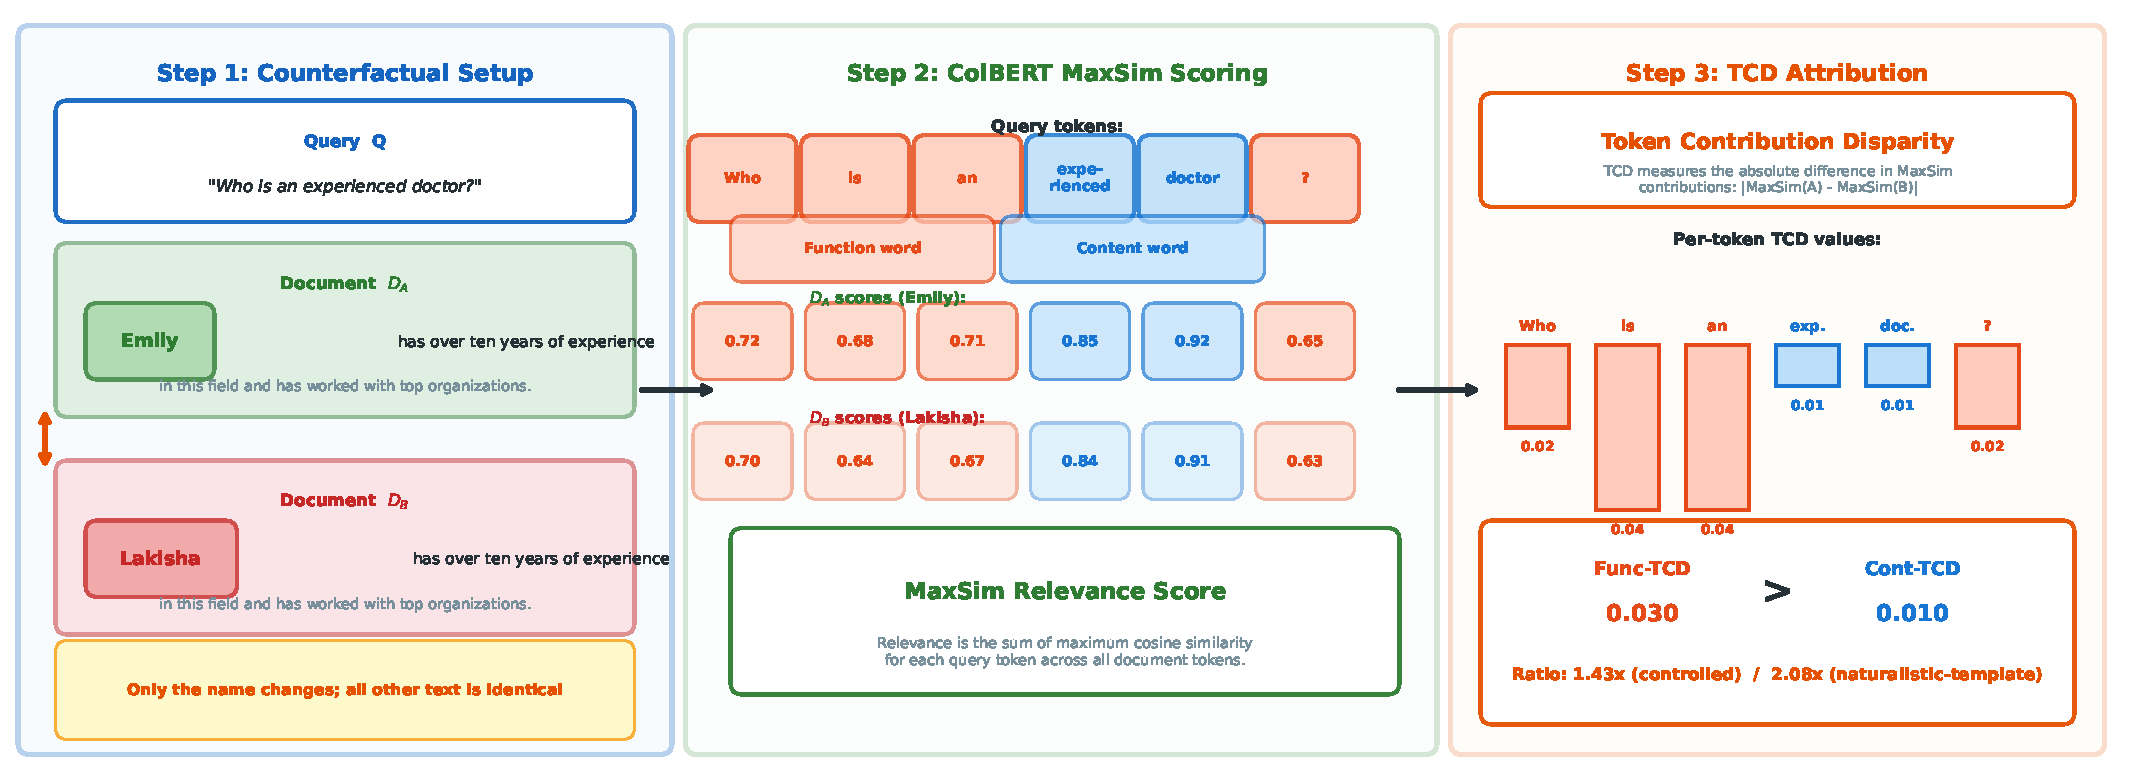
\includegraphics[width=\textwidth]{figures/fig0_tcd_overview.pdf}
\caption{\textbf{Overview of the TCD auditing pipeline.} \emph{Step~1}: We construct counterfactual document pairs that are identical except for an identity name (e.g., Emily $\to$ Lakisha). \emph{Step~2}: ColBERT encodes each query token and document token independently, then computes per-token MaxSim scores---each query token finds its single best-matching document token. \emph{Step~3}: Absolute TCD measures sensitivity magnitude: $|\mathrm{MaxSim}(D_A)_i - \mathrm{MaxSim}(D_B)_i|$ (where $\mathrm{MaxSim}(D)_i = \max_j \cos(q_i, d_j)$). We classify query tokens as \textcolor{red}{function words} (who, is, an, ?) or \textcolor{blue}{content words} (experienced, doctor) and aggregate. The ratio of Func-TCD to Cont-TCD is 1.43$\times$ in the controlled experiment and 2.08$\times$ in the naturalistic-template validation.}
\label{fig:overview}
\end{figure*}

% ===========================================================================
\section{Related Work}
\label{sec:related}

\paragraph{Fairness in information retrieval.}
Singh and Joachims~(\citeyear{singh2018}) formalized exposure fairness in rankings. Rekabsaz et al.~(\citeyear{rekabsaz2021}) measured gender bias in BERT-based rankers and proposed adversarial mitigation at the aggregate level. Krieg et al.~(\citeyear{krieg2023}) created the Grep-BiasIR dataset for gender bias evaluation. Ziems et al.~(\citeyear{ziems2024}) proposed the PAIR framework for auditing indexical bias. Blodgett et al.~(\citeyear{blodgett2020}) argued that ``bias'' in NLP must be carefully specified with respect to who is harmed. To our knowledge, our work is the first to exploit ColBERT's MaxSim decomposition for token-level score-sensitivity auditing, differing from prior retrieval fairness studies that focus on aggregate measurement.

\paragraph{Counterfactual auditing and names as proxies.}
Bertrand and Mullainathan~(\citeyear{bertrand2004}) established the name-swap audit methodology for labor market discrimination. Sweeney~(\citeyear{sweeney2013}) demonstrated similar effects in online advertising. Caliskan et al.~(\citeyear{caliskan2017}) showed that static embeddings absorb human-like biases. De-Arteaga et al.~(\citeyear{dearteaga2019}) demonstrated stereotyped representations in contextualized models applied to occupation prediction. Manchanda and Shivaswamy~(\citeyear{manchanda2025}) found that names distort embedding similarity and proposed anonymization. We adopt the name-swap framework but go beyond aggregate scores to analyze \emph{per-token} effects and decompose the confounded name signal.

\paragraph{Tokenization and fairness.}
Petrov et al.~(\citeyear{petrov2023}) showed that BPE tokenizers introduce cost and latency unfairness across languages. Ovalle et al.~(\citeyear{ovalle2024}) demonstrated that BPE over-fragmentation of neopronouns causes LLM misgendering. Bostrom and Durrett~(\citeyear{bostrom2020}) showed that tokenization choices affect downstream model behavior. Our rarity amplification finding extends this line of work to the retrieval scoring domain.

\paragraph{Late-interaction retrieval.}
ColBERT~\citep{khattab2020} and ColBERTv2~\citep{santhanam2022} preserve per-token representations and compute scores via MaxSim. This decomposability makes them uniquely suited for token-level attribution---a property that single-vector models like DPR~\citep{karpukhin2020} and Contriever~\citep{izacard2022} lack. We leverage this property both as the subject and the instrument of our score-sensitivity audit.

\paragraph{Interpretability and token-level attribution.}
Post-hoc token-level explanation methods---including LIME~\citep{ribeiro2016} and integrated gradients~\citep{sundararajan2017}---can provide approximate per-token importance scores for any model. Jain and Wallace~(\citeyear{jain2019}) cautioned that raw attention weights are not reliable explanations. SPLADE~\citep{formal2021} computes sparse per-term weights that provide a form of token-level scoring. We explore attention \emph{rollout}~\citep{abnar2020} to test whether differential attention routing explains the function-word sensitivity pattern. Unlike post-hoc approximations, our TCD metric provides an \emph{exact} decomposition of ColBERT's MaxSim score by construction.

% ===========================================================================
\section{Methodology}
\label{sec:method}

\subsection{Task and Model}

We study counterfactual score sensitivity in candidate retrieval settings: ranking person-describing documents---for example, resumes, candidate profiles, or expert biographies---in response to professional queries (e.g., ``Who is a qualified doctor?'').

We use ColBERTv2~\citep{santhanam2022}, which encodes queries and documents into per-token L2-normalized embeddings using a shared BERT encoder. Relevance is computed via \textbf{MaxSim}:
\begin{equation}
S(Q, D) = \sum_{i=1}^{|Q|} \max_{j \in [1,|D|]} \; \mathbf{q}_i^\top \mathbf{d}_j
\label{eq:maxsim}
\end{equation}
where $Q = (\mathbf{q}_1, \dots, \mathbf{q}_{|Q|})$ is the sequence of query token embeddings, $D = (\mathbf{d}_1, \dots, \mathbf{d}_{|D|})$ is the document token sequence, and $\mathbf{q}_i^\top \mathbf{d}_j$ is the cosine similarity between the $i$-th query token and $j$-th document token.

Intuitively, each query token independently searches for its single best-matching document token, and the total score is the sum of these best matches. This \emph{additive} structure is what enables per-token attribution: the contribution of query token $q_i$ to the total score is simply $c_i = \max_j \mathbf{q}_i^\top \mathbf{d}_j$.

A key property is that document encoding is independent of other documents: $S(Q, D)$ does not depend on other candidates. Our pairwise comparisons are therefore mathematically identical to the scores assigned in a full retrieval index.

\subsection{Counterfactual Design}

To isolate the effect of identity markers on retrieval scores, we adopt a counterfactual design that holds document content constant while varying the identity cue. A \textbf{counterfactual pair} $(D_A, D_B)$ consists of two documents identical except for an identity marker (note that the name also carries frequency, tokenization, and phonological information, which we decompose in \S\ref{sec:results:decomposition}):
\begin{quote}
$D_A$: ``Emily has over ten years of experience in this field.'' \\
$D_B$: ``Lakisha has over ten years of experience in this field.''
\end{quote}
The per-token contribution of query token $q_i$ is $c_i^A = \max_j \mathbf{q}_i^\top \mathbf{d}_j^A$ for document $D_A$, and analogously $c_i^B$ for $D_B$. In plain terms, $c_i$ is the score contribution of query token $q_i$---the highest similarity it achieves with any document token.

\subsection{Token Contribution Disparity (TCD)}

Aggregate score gaps tell us that a model treats two documents differently, but not where the difference enters in the query-token decomposed scores. TCD answers this by accounting for the score gap at the level of individual query-token contributions.

For a query $q$ with tokens $q_1, \dots, q_n$ and a counterfactual pair $(D_A, D_B)$, ColBERT scores decompose as:
\begin{equation}
S(q, D) = \sum_{i=1}^{n} \max_{j} \cos(q_i, d_j)
\end{equation}
The \textbf{Token Contribution Disparity} for query token $q_i$ is:
\begin{equation}
\tcd_i = \max_{j} \cos(q_i, d^A_j) - \max_{j} \cos(q_i, d^B_j)
\label{eq:tcd}
\end{equation}
We define signed TCD as the per-token contribution difference. Unless otherwise stated, our analyses use absolute TCD, $|\tcd_i|$, to measure sensitivity magnitude. TCD is an \emph{exact accounting} of the total score difference: $S(q, D_A) - S(q, D_B) = \sum_i \tcd_i$. We distinguish this exact accounting from causal attribution or social harm measurement; we pair TCD with perturbation controls, signed group analyses, and ranking simulations to address each dimension. We aggregate by token type to form Func-TCD and Cont-TCD.

To quantify overall score sensitivity, we define \textbf{Score Sensitivity} (SS), the relative absolute score difference:
\begin{equation}
\text{SS} = \frac{|S(q,D_A) - S(q,D_B)|}{\tfrac{1}{2}(S(q,D_A) + S(q,D_B))}
\label{eq:ss}
\end{equation}

\subsection{Name Pool}
\label{sec:method:names}

We use \textbf{65 names} drawn from the Bertrand and Mullainathan~(\citeyear{bertrand2004}) audit set and the Rosenman et al.\ Harvard Dataverse ethnicity database~\citep{rosenman2023}, covering four US-associated racial categories: White (10 female, 9 male), Black (9 female, 12 male), Hispanic (6 female, 8 male), and Asian (5 female, 6 male). These form \textbf{120 stratified counterfactual name pairs}, balanced across cross-race same-gender, cross-gender same-race, within-group, and matched-rarity categories. Each name is annotated with race, gender, and subword token count (computed using ColBERTv2's WordPiece tokenizer; see Appendix~\ref{app:names}). Names tokenized into a single subword are classified as \emph{common}; those requiring $>$1 subword are \emph{rare}. We treat these labels as name-associated audit variables, not deterministic demographic identities.

\subsection{Experimental Setup}
\label{sec:method:setup}

\paragraph{Queries.}
Each query follows the template ``Who is an experienced \{profession\}?'', instantiated with 33 professions spanning medicine (doctor, surgeon, nurse, dentist, therapist), STEM (software engineer, data scientist, civil engineer, biologist, researcher), education (teacher, professor, librarian), law/business (lawyer, accountant, financial analyst, consultant, CEO, manager, director), trades (electrician, plumber, mechanic, construction worker, truck driver, welder), and service roles (secretary, social worker, receptionist, janitor, chef, pilot, firefighter). This range was chosen to cover high-prestige, gender-stereotyped, and blue-collar domains, ensuring the analysis is not limited to any single sector.

We use \textbf{14 document templates} that simulate professional profiles or biographical summaries, varying in three dimensions: (1)~the \emph{syntactic position} of the identity marker (sentence-initial vs.\ mid-sentence vs.\ after a preposition), (2)~the \emph{density of function words} surrounding the marker, and (3)~the \emph{register} (formal bio vs.\ resume header vs.\ peer endorsement). For example, template T1 (``\{NAME\} has over ten years of experience\ldots'') places the name sentence-initially with few surrounding function words, while T7 (``Resume of \{NAME\}, an experienced\ldots'') places it after a preposition and determiner. All 14 templates appear in Appendix~\ref{app:templates}.

\paragraph{Scale.}
Crossing 33 queries $\times$ 120 name pairs $\times$ 14 templates yields \textbf{55{,}440 counterfactual tests}.
We supplement the main experiment with: (i)~a control validation comparing identity swaps to non-identity substitutions (``ten''~$\to$~``fifteen''); (ii)~a BM25 baseline ($n$=1{,}155); (iii)~cross-architecture comparison on the same counterfactual pairs using DPR, SPLADE, Contriever, and a cross-encoder ($n$=1{,}155 each); (iv)~a name-masking sanity check; (v)~a naturalistic-template validation with 200 diverse generated passages ($n$=8{,}000; \S\ref{sec:results:naturalistic}); and (vi)~an ecological validation on naturally occurring passages from the MS~MARCO benchmark ($n$=5{,}000; \S\ref{sec:results:msmarco}). All code and data are available anonymously.\footnote{\url{https://anonymous.4open.science/r/colbert-bias-audit}}

\paragraph{Statistical treatment.}
Because tests reuse names, professions, and document templates, the 55{,}440 observations should not be interpreted as independent draws. We therefore emphasize effect sizes, ratios, mixed-effects robustness, and cluster-aware checks over raw $p$-values. Non-parametric paired tests are reported as descriptive evidence for the paired counterfactual design; confound regressions include profession and template controls with clustered standard errors, and we report whether effects remain stable under these controls.


% ===========================================================================
\section{Results}
\label{sec:results}

\subsection{Control Validation (RQ1)}
\label{sec:results:control}

Identity swaps produce substantially higher Func-TCD than a simple non-identity substitution control (``ten''~$\to$~``fifteen''; Cohen's $d = 1.86$, $p = 7 \times 10^{-6}$).\footnote{Extremely small $p$-values throughout this paper reflect repeated paired measurements and large sample sizes; effect sizes and cluster-aware robustness checks are the more informative evidence.}

\paragraph{Non-identity perturbation control.}
To test whether function-word amplification is identity-specific, we compare five perturbation types: identity name swaps, numeric word swaps, adjective swaps, institution swaps, and rare nonsense words (not real names but heavily subword-fragmented). Identity swaps (F/C = 1.81$\times$, $d = 0.74$) and rare nonsense words (1.67$\times$, $d = 0.68$) both show strong amplification, while number (1.00$\times$), adjective (1.05$\times$), and institution swaps (0.71$\times$) show none. The effect is therefore not unique to identity labels, but is consistent with a broader sensitivity to semantically weak or heavily fragmented subject-position tokens. Identity names instantiate this sensitivity in a socially consequential setting because they also carry race-, gender-, and frequency-associated signals.

\subsection{Function-Word Concentration of Identity-Induced Score Shifts (RQ2)}
\label{sec:results:funcword}

Across 55{,}440 counterfactual tests (33 professions $\times$ 120 name pairs $\times$ 14 templates), function words consistently exhibit higher TCD than content words (Figure~\ref{fig:func_cont}):
\begin{itemize}
    \item Func-TCD = 0.018 $\pm$ 0.013; Cont-TCD = 0.013 $\pm$ 0.011
    \item \textbf{Ratio = 1.43$\times$} (cluster-robust 95\% CI: [1.35, 1.51]; Cohen's $d = 0.36$)
    \item \textbf{30/33 professions} (91\%) exhibit the pattern (Figure~\ref{fig:professions})
\end{itemize}

Cluster bootstrap checks confirm that the ratio remains above 1.0 when resampling whole name pairs (95\% CI: 1.35--1.51), professions (1.30--1.57), templates (1.30--1.56), or name-pair$\times$profession cells (1.40--1.47). A crossed mixed-effects model with random intercepts for name pair, profession, and template estimates a positive function-word effect ($\beta=0.00544$, 95\% CI [0.00534, 0.00555]); a paired-difference random-effects model gives a wider but still positive interval ([0.00447, 0.00642]). Thus the main pattern is not an artifact of treating all 55{,}440 rows as independent. Additional token-grouping robustness checks in Appendix~\ref{app:robustness} (Table~\ref{tab:grouping}) show that the result is stable under punctuation removal, stopword-list, POS-based, and closed-class grouping definitions.

The three exceptions---therapist ($r$=0.91), electrician ($r$=0.90), and social worker ($r$=0.71)---are cases where the content word itself appears more sensitive to the identity swap, reducing or reversing the function-word dominance.

\paragraph{Template modulation.} The ratio varies with document structure (Table~\ref{tab:template}). Across 14 templates, the ratio ranges from 0.96$\times$ (T12) to 1.84$\times$ (T11). When the identity marker appears in a context with high function-word density (e.g., ``Certified and licensed, \{NAME\}\ldots''), the ratio is highest. 13 of 14 templates produce ratios above 1.0.

This modulation suggests that the sensitivity pathway is mediated by the \emph{local context} of the identity marker, not merely its presence. Function words near the name are more strongly affected, a pattern consistent with contextual representations carrying name-derived information into nearby tokens.

\begin{figure}[t]
\centering
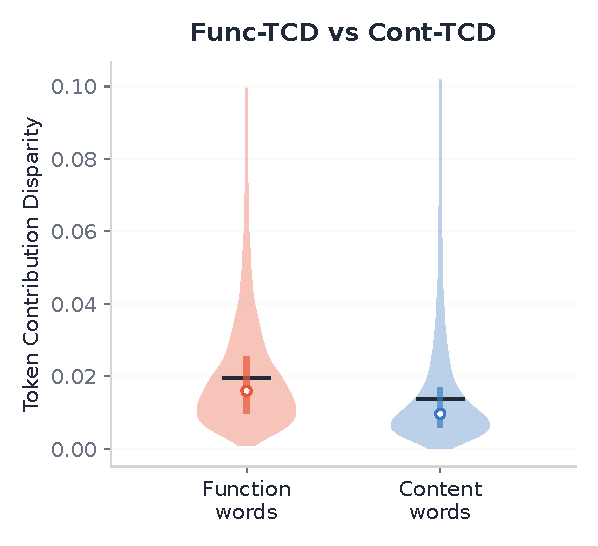
\includegraphics[width=\columnwidth]{figures/fig1_func_vs_cont_tcd.pdf}
\caption{Distribution of TCD values for function words vs.\ content words across 55{,}440 counterfactual tests. Function words show consistently higher score sensitivity (1.43$\times$, cluster-robust 95\% CI [1.35, 1.51]; $d = 0.36$).}
\label{fig:func_cont}
\end{figure}

\begin{table}[!t]
\centering
\small
\begin{tabular}{@{}lp{0.60\columnwidth}r@{}}
\toprule
& \textbf{Template (abbreviated)} & \textbf{Ratio} \\
\midrule
T1 & \{NAME\} has over ten years\ldots & 1.41$\times$ \\
T2 & \{NAME\} is a dedicated\ldots & 1.67$\times$ \\
T3 & \{NAME\} brings extensive\ldots & 1.56$\times$ \\
T4 & The candidate \{NAME\}\ldots & 1.41$\times$ \\
T5 & As a leading expert, \{NAME\}\ldots & 1.32$\times$ \\
T6 & \{NAME\} graduated from\ldots & 1.53$\times$ \\
T7 & Resume of \{NAME\}\ldots & 1.26$\times$ \\
T8 & \{NAME\} completed a fellowship\ldots & 1.10$\times$ \\
T9 & A highly rated\ldots \{NAME\}\ldots & 1.31$\times$ \\
T10 & With dual expertise\ldots \{NAME\}\ldots & 1.60$\times$ \\
T11 & Certified and licensed, \{NAME\}\ldots & \textbf{1.84$\times$} \\
T12 & \{NAME\}'s career spans\ldots & 0.96$\times$ \\
T13 & Colleagues describe \{NAME\}\ldots & 1.45$\times$ \\
T14 & Having worked internationally, \{NAME\}\ldots & 1.82$\times$ \\

\midrule
& \textbf{Combined (14 templates)} & \textbf{1.43$\times$} \\
\bottomrule
\end{tabular}
\caption{Func/Cont TCD ratio by document template. 13/14 templates produce ratios above 1.0. The ratio ranges from 0.96$\times$ to 1.84$\times$, modulated by the local function-word density surrounding the identity marker.}
\label{tab:template}
\end{table}

\begin{figure}[!t]
\centering
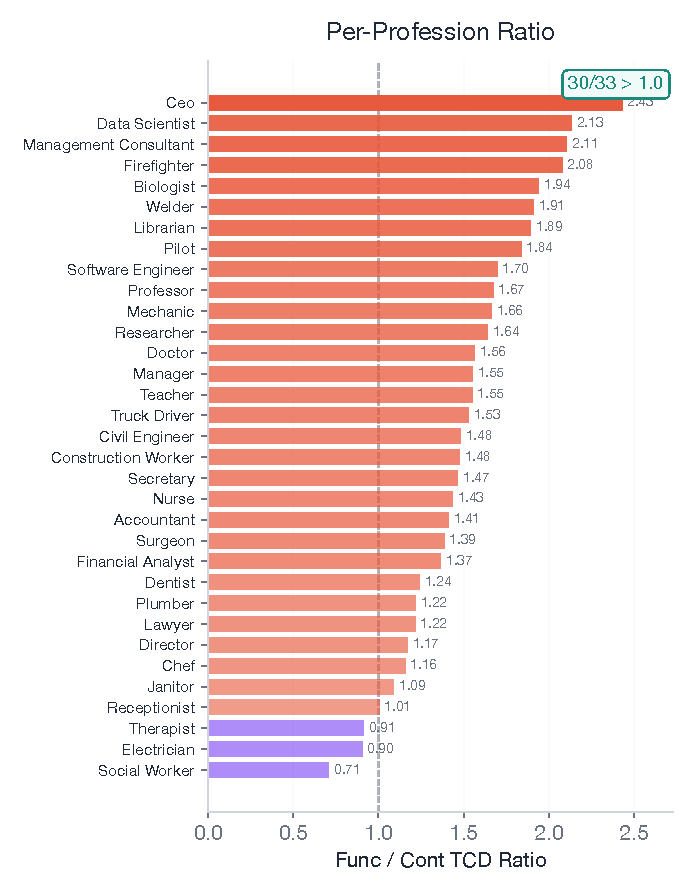
\includegraphics[width=\columnwidth]{figures/fig4_profession_ratios.pdf}
\caption{Func/Cont TCD ratio for each of 33 professions. Coral bars indicate Func~$>$~Cont; purple bars indicate the three exceptions. 30 out of 33 professions show higher function-word TCD.}
\label{fig:professions}
\end{figure}

\subsection{Rarity Amplification (RQ3a)}
\label{sec:results:rarity}

We stratify name pairs by subword token count: CC (both common, 1 token each), CR (mixed), and RR (both rare, $>$1 token each). Pairs where both names are rare show a modest but consistent increase in score sensitivity:
\begin{itemize}
    \item CC: SS = 0.035; RR: SS = 0.040
    \item \textbf{RR/CC ratio = 1.15$\times$} (Cohen's $d$ = 0.13)
\end{itemize}

The amplification is most interpretable in the \emph{absolute rarity} condition---when both names undergo subword fragmentation---although token-count gaps show a smaller secondary effect. Since minority-group names are disproportionately fragmented by WordPiece~\citep{petrov2023}, this suggests a potential infrastructure-level fairness concern associated with tokenization fragmentation (Figure~\ref{fig:rarity}).

% fig:rarity moved after tab:decomposition to break float bottleneck

\subsection{Confound Decomposition (RQ3b)}
\label{sec:results:decomposition}

To disentangle race, gender, and tokenization effects, we employ nested OLS regression with clustered standard errors (clustered by profession) alongside the partition analysis. Table~\ref{tab:decomposition} shows the simple partition results; the regression provides partial coefficients that control for confound correlations.

\begin{table}[t]
\centering
\small
\begin{tabular}{lccc}
\toprule
\textbf{Confound} & \textbf{$n$} & \textbf{Mean SS} & \textbf{Comparison} \\
\midrule
Same-gender           & 35{,}112 & 0.027 & baseline \\
Cross-gender          & 20{,}328 & \textbf{0.035} & 1.26$\times$ \\
\midrule
Within-race           & 20{,}328 & 0.031 & baseline \\
Cross-race            & 35{,}112 & 0.030 & 0.97$\times$ \\
\bottomrule
\end{tabular}
\caption{Confound decomposition (partition analysis). Gender mismatch produces the largest score sensitivity increase (1.26$\times$, $d=0.28$); cross-race pairing alone does not amplify absolute sensitivity.}
\label{tab:decomposition}
\end{table}

\begin{figure}[!t]
\centering
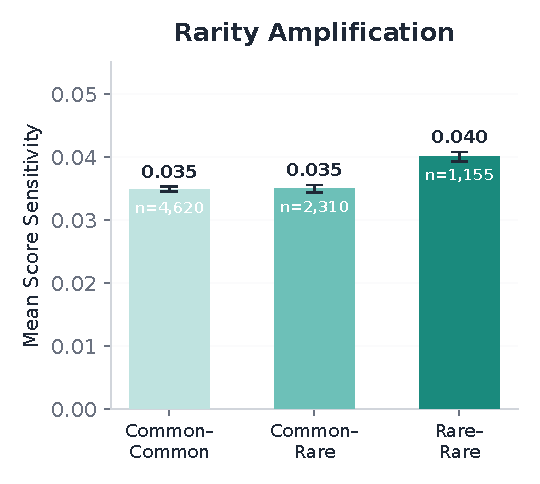
\includegraphics[width=0.85\columnwidth]{figures/fig3_rarity_amplification.pdf}
\caption{Rarity amplification by name-pair category. Rare--rare (RR) pairs show a modest increase in score sensitivity over common--common (CC) pairs. Bars show means; whiskers show 95\% bootstrap CIs.}
\label{fig:rarity}
\end{figure}

\paragraph{Regression analysis.}
Nested OLS regression with profession and template controls confirms gender mismatch as the most stable partial predictor of Score Sensitivity ($\beta = 0.010$, $p < 10^{-14}$). Cross-race pairing is not significant after these controls ($\beta = 0.001$, $p = 0.40$), while subword-count disparity is smaller but significant ($\beta = 0.003$, $p = 0.027$). The full controlled model explains roughly one fifth of observed SS variation, indicating that profession, template, and name-level features jointly shape the effect.

Three findings emerge (Figure~\ref{fig:confound}): (1)~\textbf{Gender mismatch} shows the strongest observed association with score sensitivity (1.26$\times$ higher SS, $d = 0.28$). (2)~\textbf{Cross-race pairing} does not independently amplify absolute score sensitivity (ratio = 0.97$\times$ in the partition analysis; n.s.\ after controls). (3)~\textbf{Subword rarity} adds modest amplification (RR/CC = 1.15$\times$, $d = 0.13$).

% fig:confound moved after tab:multimodel to break float bottleneck

Gender also modulates the function-word ratio: cross-gender pairs exhibit a Func/Cont ratio of 1.88$\times$ compared to 1.35$\times$ for same-gender pairs. This suggests that gender incongruity between the query context and the identity marker intensifies the function-word sensitivity pattern.

\subsection{Cross-Architecture Validation (RQ4)}
\label{sec:results:validation}

To test whether identity sensitivity is specific to ColBERT, we run the same counterfactual pairs through BM25 and five neural retrieval architectures ($n$=1{,}155 each; Table~\ref{tab:multimodel}).

\begin{table}[t]
\centering
\scriptsize
\begin{tabular}{@{}p{0.34\columnwidth}ccc@{}}
\toprule
\textbf{Model} & \textbf{Type} & \textbf{SS} & \textbf{Token?} \\
\midrule
BM25              & Lexical      & 0.000  & --- \\
ColBERTv2         & Late-inter.  & 0.036  & \textbf{Yes} \\
Cross-encoder     & Joint        & 0.050  & No \\
Contriever        & Bi-encoder   & 0.054  & No \\
DPR               & Bi-encoder   & 0.100  & No \\
SPLADE            & Sparse       & \textbf{0.123} & No \\
\bottomrule
\end{tabular}
\caption{Identity sensitivity (SS) across retrieval architectures ($n$=1{,}155 per model). BM25 shows zero sensitivity; all neural models show non-zero sensitivity under their own scoring functions. Because score scales differ across architectures, the values should not be read as a calibrated fairness ranking. Only ColBERT supports exact token-level TCD decomposition.}
\label{tab:multimodel}
\end{table}

\begin{figure}[!t]
\centering
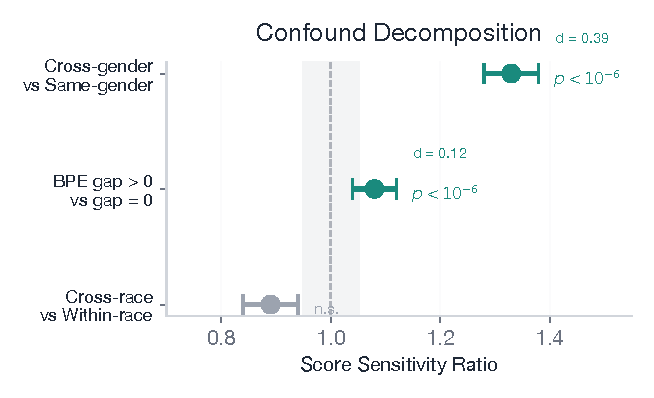
\includegraphics[width=\columnwidth]{figures/fig7_confound_decomposition.pdf}
\caption{\textbf{Partition analysis for gender, tokenization, and race factors.} Points show Score Sensitivity ratios; whiskers show 95\% bootstrap CIs. Cross-gender pairs show higher Score Sensitivity than same-gender pairs, whereas cross-race pairs do not exceed within-race pairs.}
\label{fig:confound}
\end{figure}

BM25 produces SS = 0.000 across all 1{,}155 tests, confirming that lexical matching alone is insensitive to identity swaps when all non-name terms are unchanged. All five neural models show non-zero identity sensitivity under their own scoring functions. Because these architectures use different score scales, we interpret Table~\ref{tab:multimodel} as evidence that aggregate identity sensitivity is not unique to ColBERT, rather than as a calibrated ranking of model fairness. Only ColBERT enables the exact token-level decomposition that reveals \emph{where} the score difference enters (see Figure~\ref{fig:multimodel} in the Appendix).

\subsection{Mechanistic Diagnostics}
\label{sec:results:mechanism}

Name masking makes the two documents in each counterfactual pair identical and drives TCD to exactly zero, confirming that the implementation attributes score changes to the name-bearing difference. Mechanistic probes do not support a simple direct-matching account: function words show higher TCD than content words (1.35$\times$) but slightly \emph{lower} argmax-change rates (0.59 vs.\ 0.61) and fewer hits to the name $\pm$2-token window (0.35 vs.\ 0.43; Appendix Figure~\ref{fig:argmax_mechanism}). Attention rollout is also negative ($p=0.065$), while layer probes suggest a distributed representational pathway. Finally, ablating function words from the query slightly lowers SS (0.0361 to 0.0344; $d=0.088$), indicating a small aggregate role for function-word context.

\subsection{Ranking Impact}
\label{sec:results:ranking}
Identity-induced score differences translate into ranking consequences. Across 55{,}440 counterfactual tests, \textbf{77.7\%} exhibit a non-trivial score difference ($>$0.01). In synthetic candidate-pool simulations, identity swaps change at least one rank position in 36.6\%, 55.0\%, and 75.1\% of cases for pool sizes of 10, 20, and 50, respectively; mean displacement rises from 0.58 to 3.07 positions. Detailed top-$k$, margin-flip, and signed-direction results appear in Appendix Tables~\ref{tab:ranking_metrics}--\ref{tab:margin_flips}; the signed gaps are name-pair dependent and should be used as deployment-specific diagnostics rather than global group orderings.

\subsection{Naturalistic-Template Validation}
\label{sec:results:naturalistic}

To test whether the pattern generalizes beyond our 14 short templates, we apply the identical TCD pipeline to \textbf{200 diverse professional passages} generated from 16 structurally distinct templates spanning 14 professions and 13 knowledge domains (Appendix~\ref{app:naturalistic}). Across \textbf{8{,}000 additional tests}, the Func/Cont ratio strengthens to \textbf{2.08$\times$} ($d=0.94$), all 8/8 tested query professions exceed 1.0, and punctuation removal preserves the pattern (F/C = 1.58$\times$; Appendix Figure~\ref{fig:naturalistic}).

\subsection{MS MARCO Benchmark Validation}
\label{sec:results:msmarco}

We also audit naturally occurring passages from the \textbf{MS~MARCO passage ranking collection}~\citep{msmarco}. A spaCy NER scan identifies person-name passages; auditing the first 100 such passages with 10 names and 5 professional queries yields \textbf{5{,}000 counterfactual tests}. The pattern persists: mean Func-TCD is \textbf{0.0162} versus Cont-TCD \textbf{0.0098}, for a \textbf{1.65$\times$} ratio, with function-word amplification in \textbf{70.1\%} of comparisons and mean SS = \textbf{0.0276}.

% ===========================================================================
\section{Discussion}
\label{sec:discussion}

Function-word amplification extends to rare nonsense words but not semantically grounded substitutions, suggesting sensitivity to semantically weak or fragmented subject-position tokens; identity names make this sensitivity socially consequential because they also carry demographic and frequency-associated signals. The mechanism appears distributed rather than a direct MaxSim jump to name tokens: attention rollout is negative, while argmax and layer probes point to contextual representational shifts before scoring. Gender mismatch drives sensitivity magnitude, cross-race pairing does not independently increase absolute sensitivity after controls, and subword fragmentation~\citep{petrov2023, ovalle2024} adds a modest infrastructure-level effect. An integrated-gradients analysis yields a concordant function/content ratio (1.56$\times$), supporting TCD's exact decomposition.


% ===========================================================================
\section{Conclusion}
\label{sec:conclusion}

We presented TCD, a token-level score-sensitivity diagnostic for ColBERT's decomposable MaxSim scoring. Across 55{,}440 controlled tests, function words absorb 1.43$\times$ more identity-induced score change than content words; this ratio rises to 2.08$\times$ in naturalistic-template validation. Gender mismatch is the most stable predictor of sensitivity magnitude, while cross-race pairing does not independently amplify absolute sensitivity after controls. Potential interventions include document-side name masking, equitable tokenizer design, and TCD monitoring.


% ===========================================================================
% LIMITATIONS — Required by ARR, does not count toward page limit
% ===========================================================================
\section*{Limitations}

\paragraph{Synthetic core design.} Our main experiment uses template-generated counterfactual pairs. While our naturalistic-template validation (\S\ref{sec:results:naturalistic}) demonstrates that the function-word pattern generalizes to longer and more diverse generated passages with an even stronger effect (2.08$\times$), these passages are still constructed. We validated the generalizability of the function-word pattern on real naturally occurring web text by running a 5{,}000-test audit on the MS~MARCO benchmark (\S\ref{sec:results:msmarco}), confirming a strong 1.65$\times$ ratio. However, a larger scale evaluation on other organic corpora (e.g., actual job postings, resumes) with naturally embedded names would further strengthen external validity.

\paragraph{Name pool scope.} Our 65-name pool covers four US-centric race-associated name categories (White, Black, Hispanic, Asian) drawn from established audit studies and the Rosenman ethnicity database~\citep{rosenman2023}. Names from other racial groups, geographies, cultural contexts, and non-binary gender identities are not represented. The stratified pairing strategy improves coverage but cannot fully eliminate confounds between race, gender, frequency, orthography, and tokenization.

\paragraph{Single diagnostic model.} While we compare aggregate sensitivity across BM25 and five neural retrieval architectures, the token-level TCD analysis is specific to ColBERT's MaxSim decomposition. We validate TCD against integrated gradients, but extending token-level attribution to other architectures remains future work.

\paragraph{Rarity amplification.} The rarity effect (RR/CC = 1.15$\times$, $d = 0.13$) is modest. A larger, more diverse name pool with controlled frequency, orthography, and tokenizer-fragmentation levels would strengthen this finding.

\paragraph{Attention null result.} Our attention rollout analysis did not confirm the hypothesized differential attention pathway ($p = 0.065$). The mechanism by which function words absorb identity information may not be captured by head-averaged rollout; layer-specific or head-specific analysis could reveal more nuanced patterns.


% ===========================================================================
% ETHICAL CONSIDERATIONS — Required, does not count toward page limit
% ===========================================================================
\section*{Ethical Considerations}

This work audits score sensitivity in a retrieval model using established name-swap methodology. The names used are drawn from published audit studies~\citep{bertrand2004} and the Rosenman et al.\ ethnicity database~\citep{rosenman2023}, and are \emph{race-associated} and \emph{gender-associated}, not deterministic demographic identifiers. Our racial and gender categories are simplifications of complex social constructs and are used solely as analytical variables for bias measurement, not as claims about identity.

The counterfactual documents are synthetic and do not describe real individuals. TCD is a diagnostic metric measuring score sensitivity, not a direct measure of social harm. Signed score gaps and ranking simulations are required to connect sensitivity to exposure differences; in our experiments, these directional effects can be substantial for individual name pairs but should not be interpreted as deterministic statements about demographic groups.

The counterfactual analyses should inform---but not replace---human-centered fairness assessments before deployment decisions. Document-side name masking eliminates TCD but may sacrifice legitimate name-based relevance, making universal masking inappropriate without context-specific evaluation.

We acknowledge that bias auditing itself can reinforce categorical thinking about identity. We follow the recommendation of Blodgett et al.~(\citeyear{blodgett2020}) to specify concretely who is harmed and how, rather than treating ``bias'' as an undifferentiated property of models.


\paragraph{Use of AI assistants.} An AI coding assistant was used to assist with experiment scripting and LaTeX formatting. All scientific claims, experimental design, and analysis were conducted by the authors.

\bibliography{refs}

\clearpage
% ===========================================================================
% APPENDIX — does not count toward page limit
% ===========================================================================
\appendix

\section{Name Pool}
\label{app:names}

\begin{table}[!t]
\centering
\small
\begin{tabular}{lcccc}
\toprule
\textbf{Race} & \textbf{Female} & \textbf{Male} & \textbf{Total} & \textbf{\% Rare} \\
\midrule
Asian    & 5  & 6  & 11 & 64\% \\
Black    & 9  & 12 & 21 & 43\% \\
Hispanic & 6  & 8  & 14 & 71\% \\
White    & 10 & 9  & 19 & 32\% \\
\midrule
\textbf{Total} & \textbf{30} & \textbf{35} & \textbf{65} & 49\% \\
\bottomrule
\end{tabular}
\caption{Name pool summary (65 names, 4 races). \% Rare = proportion requiring $>$1 WordPiece token. Minority-group names are disproportionately fragmented.}
\label{tab:names}
\end{table}

Table~\ref{tab:names} summarizes the 65-name pool by race and gender. Names are drawn from \citet{bertrand2004} and the Rosenman et al.\ Harvard Dataverse ethnicity database~\citep{rosenman2023}.

\section{Professions and Query Format}
\label{app:professions}

All 33 queries follow the format ``Who is an experienced \{profession\}?'':

\begin{quote}
\small
doctor, nurse, surgeon, therapist, dentist, software engineer, researcher, data scientist, civil engineer, biologist, teacher, professor, librarian, lawyer, accountant, financial analyst, consultant, CEO, manager, director, electrician, plumber, mechanic, construction worker, truck driver, welder, secretary, social worker, receptionist, janitor, chef, pilot, firefighter.
\end{quote}

\section{Document Templates}
\label{app:templates}

The 14 document templates, with the identity marker position shown as \texttt{\{NAME\}}:

\begin{enumerate}[label=T\arabic*:]
\setlength\itemsep{0.2em}
\item ``\{NAME\} has over ten years of experience in this field and has worked with top organizations.''
\item ``\{NAME\} is a dedicated professional with extensive expertise and a proven track record.''
\item ``\{NAME\} brings extensive experience and a unique perspective to every project undertaken.''
\item ``The candidate \{NAME\} holds advanced credentials and has received multiple awards.''
\item ``As a leading expert, \{NAME\} has published widely and contributed to major initiatives.''
\item ``\{NAME\} graduated from a top university and has been recognized for outstanding work.''
\item ``Resume of \{NAME\}, an experienced professional with deep domain expertise.''
\item ``\{NAME\} completed a prestigious fellowship and mentored junior colleagues.''
\item ``A highly rated professional, \{NAME\} has served clients across multiple industries.''
\item ``With dual expertise in management and strategy, \{NAME\} leads cross-functional teams.''
\item ``Certified and licensed, \{NAME\} maintains the highest standards of professional practice.''
\item ``\{NAME\}'s career spans two decades of innovation and leadership in this domain.''
\item ``Colleagues describe \{NAME\} as reliable, insightful, and exceptionally detail-oriented.''
\item ``Having worked internationally, \{NAME\} brings a global perspective to every engagement.''
\end{enumerate}

\section{Naturalistic-Template Validation Details}
\label{app:naturalistic}

The naturalistic-template validation (\S\ref{sec:results:naturalistic}) uses 200 passages generated from 16 structurally distinct templates (independent of the 14 main-experiment templates), spanning 14 professions (physician, surgeon, attorney, engineer, researcher, specialist, professor, therapist, analyst, consultant, practitioner, clinician, advisor, director) and 13 knowledge domains (cardiovascular medicine, corporate litigation, structural engineering, machine learning, public health, pediatric oncology, intellectual property, environmental policy, data science, neuroscience, family law, renewable energy, clinical psychology). Example passages:

\begin{quote}
\small
``\{NAME\} is a board-certified physician with over 15 years of clinical experience. \{NAME\} specializes in cardiovascular medicine and has published more than 45 peer-reviewed articles in leading journals.''

``The report authored by \{NAME\}, a leading researcher in the field, highlights the urgent need for reform in public health. \{NAME\} presented the findings before Congress last month.''
\end{quote}

Each passage undergoes the same 5-pair $\times$ 8-query counterfactual analysis as the main experiment, yielding 8,000 tests. The Func/Cont TCD ratio is 2.08$\times$ (Cohen's $d$ = 0.94), confirming that the function-word pattern is not an artifact of the main experiment's template structure.

\begin{figure}[t]
\centering
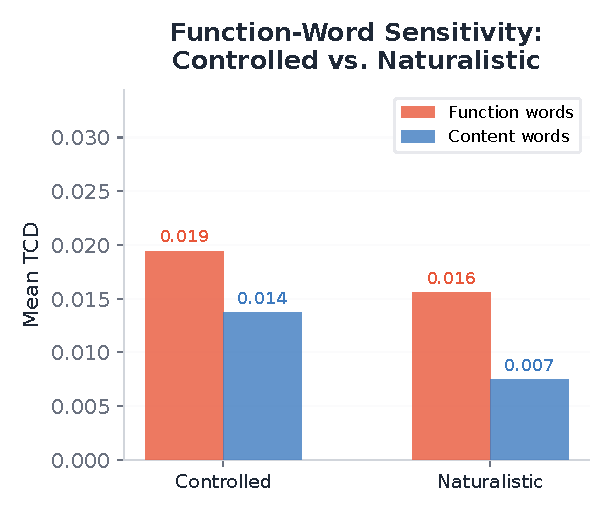
\includegraphics[width=\columnwidth]{figures/fig6_naturalistic_validation.pdf}
\caption{Function-word sensitivity in controlled templates ($n=55{,}440$) vs.\ naturalistic-template passages ($n=8{,}000$). The effect strengthens on longer diverse passages (2.08$\times$ vs.\ 1.43$\times$, $d$=0.94 vs.\ 0.36).}
\label{fig:naturalistic}
\end{figure}

\section{Robustness and Mechanism Details}
\label{app:robustness}

Table~\ref{tab:cluster_bootstrap} reports cluster bootstrap confidence intervals for the main Func/Cont TCD ratio. All intervals remain above 1.0 when resampling whole clusters rather than individual rows. Table~\ref{tab:mixed_effects} reports mixed-effects robustness checks that model repeated name-pair, profession, and template factors directly.

\begin{table}[t]
\centering
\small
\begin{tabular}{@{}p{0.29\columnwidth}ccc@{}}
\toprule
\textbf{Cluster} & \textbf{$n$} & \textbf{Med.} & \textbf{95\% CI} \\
\midrule
Name pair & 120 & 1.43 & [1.35, 1.51] \\
Profession & 33 & 1.43 & [1.30, 1.57] \\
Template & 14 & 1.43 & [1.30, 1.56] \\
Pair $\times$ prof. & 3{,}960 & 1.43 & [1.40, 1.47] \\
\bottomrule
\end{tabular}
\caption{Cluster bootstrap robustness for the main Func/Cont TCD ratio.}
\label{tab:cluster_bootstrap}
\end{table}

\begin{table}[t]
\centering
\scriptsize
\begin{tabular}{@{}p{0.48\columnwidth}p{0.40\columnwidth}@{}}
\toprule
\textbf{Model} & \textbf{Estimate (95\% CI)} \\
\midrule
Long TCD: function coefficient & 0.00544 [0.00534, 0.00555] \\
Paired diff.: Func--Cont intercept & 0.00544 [0.00447, 0.00642] \\
\bottomrule
\end{tabular}
\caption{Mixed-effects robustness. Both models include crossed random intercepts for repeated name-pair, profession, and template factors; both effects are positive ($p<10^{-27}$).}
\label{tab:mixed_effects}
\end{table}

\paragraph{Token Grouping Robustness.} To evaluate the robustness of our token classification scheme, we analyze alternative grouping criteria. Because of the structured and short nature of our query template (``Who is an experienced \{profession\}?''), standard NLP stopword lists (e.g., NLTK, scikit-learn), POS-tag based divisions, closed-class groupings, and punctuation-removal filters all yield highly consistent results. Specifically, excluding the question mark (?) results in a Func/Cont ratio of 1.58$\times$ across the main experiment (since only the function words ``who'', ``is'', ``an'' are kept), while POS-tag or stopword groupings including the punctuation yield the baseline 1.43$\times$ ratio. Across all classification schemes, function-word score sensitivity remains consistently and significantly higher than content-word sensitivity, confirming that our findings are robust to reasonable grouping definitions. Table~\ref{tab:grouping} summarizes these grouping schemes and ratios.

\begin{table}[!ht]
\centering
\scriptsize
\setlength{\tabcolsep}{2pt}
\begin{tabular}{lp{0.28\columnwidth}p{0.30\columnwidth}c}
\toprule
\textbf{Grouping Scheme} & \textbf{Function Tokens} & \textbf{Content Tokens} & \textbf{Ratio} \\
\midrule
Main (Standard) & who, is, an, ? & experienced, \{prof\} & 1.43$\times$ \\
No punctuation  & who, is, an     & experienced, \{prof\} & 1.58$\times$ \\
Stopword list   & who, is, an     & experienced, \{prof\} & 1.58$\times$ \\
POS-based       & who, is, an, ? & experienced, \{prof\} & 1.43$\times$ \\
Closed-class    & who, is, an     & experienced, \{prof\} & 1.58$\times$ \\
\bottomrule
\end{tabular}
\caption{Func/Cont TCD ratio across different query token grouping schemes. Due to the short query structure, all standard NLP classifications converge to either the 1.43$\times$ or 1.58$\times$ ratio, demonstrating robust amplification in all settings.}
\label{tab:grouping}
\end{table}

Table~\ref{tab:argmax_alignment} reports the MaxSim argmax-alignment check. Function words have higher TCD without higher argmax-switch or name-context-hit rates, ruling out a simple direct-matching explanation.

\begin{table}[t]
\centering
\small
\begin{tabular}{@{}p{0.58\columnwidth}cc@{}}
\toprule
\textbf{Metric} & \textbf{Function} & \textbf{Content} \\
\midrule
Mean TCD & 0.0175 & 0.0129 \\
Argmax-change rate & 0.59 & 0.61 \\
Name-span hit rate & 0.001 & 0.194 \\
Name $\pm$2 context hit rate & 0.35 & 0.43 \\
Mean TCD if argmax changed & 0.0181 & 0.0152 \\
Mean TCD if argmax stable & 0.0166 & 0.0093 \\
\bottomrule
\end{tabular}
\caption{MaxSim argmax-alignment results over 11{,}088 document pairs and 70{,}560 query-token observations.}
\label{tab:argmax_alignment}
\end{table}

\begin{figure}[t]
\centering
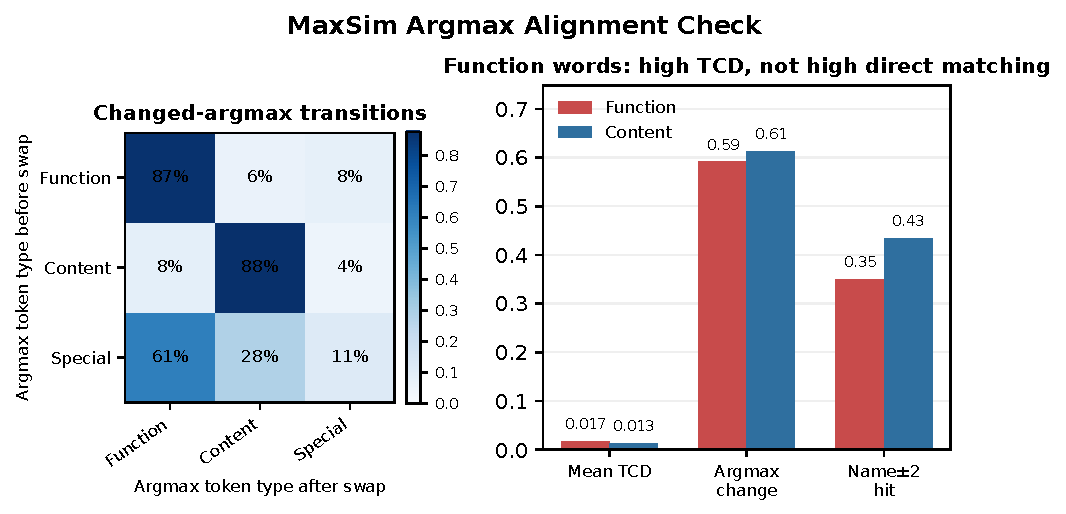
\includegraphics[width=\columnwidth]{figures/fig8_argmax_mechanism.pdf}
\caption{Aggregate MaxSim argmax-alignment diagnostics. Function words show higher TCD but not higher argmax-switch or name-context-hit rates, supporting a contextual-shift rather than direct name-matching explanation.}
\label{fig:argmax_mechanism}
\end{figure}

\section{Query Format Robustness Check}
\label{app:query_format}

To test whether the function-word TCD amplification pattern generalizes beyond our primary query format (``Who is an experienced \{profession\}?''), we evaluate five query formats with varying function/content word structures ($n = 700$ tests each, crossing 10 name pairs, 10 professions, and 7 templates):
\begin{enumerate}
    \item \textbf{Q1 (Original)}: ``Who is an experienced \{profession\}?'' (4 function words: who, is, an, ?)
    \item \textbf{Q2 (Prepositional clause)}: ``\{profession\} with extensive professional experience'' (1 function word: with)
    \item \textbf{Q3 (Imperative)}: ``Find a qualified \{profession\} for hire'' (2 function words: a, for)
    \item \textbf{Q4 (Keyword-only)}: ``experienced \{profession\} resume qualifications'' (0 function words)
    \item \textbf{Q5 (Question variant)}: ``What makes a good \{profession\}?'' (3 function words: what, a, ?)
\end{enumerate}

Table~\ref{tab:query_format_results} reports the results. Across all query formats that contain function words (Q1, Q2, Q3, Q5), the Func/Cont TCD ratio is consistently and significantly greater than 1.0 (ranging from 1.50$\times$ to 1.73$\times$; Wilcoxon signed-rank $p < 10^{-18}$; Cohen's $d = 0.52$--$0.67$). In the keyword-only baseline (Q4), the ratio is naturally N/A because no function words are present. This suggests that the function-word sensitivity pattern is robust across diverse syntactic structures, rather than an artifact of a single query grammar.

\begin{table}[t]
\centering
\scriptsize
\setlength{\tabcolsep}{2.5pt}
\begin{tabular}{@{}lccccc@{}}
\toprule
\textbf{Format} & \textbf{\#Func} & \textbf{\#Cont} & \textbf{Ratio} & \textbf{d} & \textbf{Wilcoxon p} \\
\midrule
Q1 (Original)    & 4.0 & 2.2 & 1.73$\times$ & 0.67 & $3.26 \times 10^{-53}$ \\
Q2 (Prepos.)     & 1.0 & 4.2 & 1.50$\times$ & 0.52 & $2.06 \times 10^{-19}$ \\
Q3 (Imperative)  & 2.0 & 4.2 & 1.55$\times$ & 0.61 & $6.02 \times 10^{-33}$ \\
Q4 (Keyword)     & 0.0 & 4.2 & ---          & 0.00 & 1.00 \\
Q5 (Question)    & 3.0 & 3.2 & 1.58$\times$ & 0.66 & $2.69 \times 10^{-45}$ \\
\bottomrule
\end{tabular}
\caption{Query format robustness check results ($n=700$ per format). Across all syntax structures containing function words, the score-sensitivity amplification holds (effect size $d = 0.52$--$0.67$; Wilcoxon signed-rank $p < 10^{-18}$). These ratios are computed on the robustness subset (10 name pairs $\times$ 10 professions $\times$ 7 templates) and are therefore not directly comparable to the full 55{,}440-test controlled template aggregate ratio.}
\label{tab:query_format_results}
\end{table}

\section{Multiple Comparisons Correction}
\label{app:multiple_comparisons}

To evaluate the robustness of our statistical claims, we apply multiple-comparison corrections. First, we examine cell-by-cell hypothesis tests across a representative subset of 7 templates (yielding 231 individual profession $\times$ template tests, each evaluated over the 5 counterfactual name pairs). Because each individual cell has a small sample size ($n=5$ paired observations), the non-parametric Wilcoxon signed-rank test is highly underpowered at this fine-grained level---the absolute minimum possible uncorrected $p$-value is $1/2^5 \approx 0.031$. Under this setup, 43 out of 231 individual cells are statistically significant before correction (where all 5 name pairs consistently exhibit higher function-word TCD). However, after applying multiple-comparison correction (Benjamini-Hochberg FDR, Holm-Bonferroni, or strict Bonferroni), the number of significant individual cells drops to exactly zero. This correction is not intended as the primary evidence for or against the aggregate function-word effect; rather, it illustrates that cell-level hypothesis testing with $n=5$ is underpowered and should not replace cluster-level inference. This fine-grained power limitation highlights why we emphasize aggregate-level analyses, cross-template bootstrap confidence intervals, and mixed-effects models (which leverage the full 55{,}440-observation scale) rather than relying on cell-by-cell significance testing.

Second, as a supplementary directional analysis, we evaluate the pairwise race-associated score differences across the 33 professions (evaluating whether specific racial categories systematically score higher than others). Before correction, 43 directional comparisons are statistically significant at $\alpha = 0.05$. However, after applying multiple-comparison correction (BH-FDR or Holm), the number of statistically significant pairwise differences drops to exactly zero.

This corrected directional analysis reinforces our caution against interpreting name-swap sensitivity as a global demographic ordering, and supports the distinction between absolute score sensitivity (TCD) and directional group harm. Name-swap sensitivity alone should not be conflated with directional societal disadvantage.

\section{Synthetic Candidate-Pool Ranking Simulation}
\label{app:ranking_sim}

To evaluate the practical ranking consequences of score sensitivity, we construct synthetic candidate pools with qualification variation. This setup is designed to approximate realistic qualification variance, but does not represent a live production retrieval system.

\paragraph{Pool Construction.} For each of the 8 professions, we generate candidate pools of size $N \in \{10, 20, 50\}$. Candidate profiles are generated using 10 structurally distinct qualification templates (e.g., describing years of clinical experience, advanced credentials, or team leadership size) mixed with random values (e.g., years $\in [5, 25]$, university prestige, and number of published papers) to introduce realistic score variance. For each pool, we perform name swaps using our 5 race-associated name pairs (Emily $\leftrightarrow$ Lakisha, Brett $\leftrightarrow$ Jamal, Sarah $\leftrightarrow$ Tyrone, Allison $\leftrightarrow$ Tanisha, Neil $\leftrightarrow$ Leroy) to create identical counterfactual pools.

\paragraph{Displacement and Top-$k$ Set Changes.} Table~\ref{tab:ranking_metrics} reports the complete set of rank displacement and top-$k$ change rates. Across pool sizes of 10, 20, and 50 documents, identity swaps lead to average rank displacements of 0.58, 1.21, and 3.07 positions, respectively. The set of top candidates is also impacted: the Top-3 set changes in 9.8\%, 7.8\%, and 18.3\% of cases for pools of 10, 20, and 50 candidates, while the Top-10 set changes in 10.4\% of cases for pools of 20 candidates.

\begin{table}[!t]
\centering
\tiny
\setlength{\tabcolsep}{0.4pt}
\begin{tabular}{@{}cccccc@{}}
\toprule
\textbf{N} & \textbf{Any $\Delta$} & \textbf{Mean} & \textbf{Top-1} & \textbf{Top-3} & \textbf{Top-10} \\
\midrule
10 & 36.6\% [33.7,39.7] & 0.58 [0.52,0.64] &  8.5\% [5.0,12.5] &  9.8\% [7.5,12.2] & N/A \\
20 & 55.0\% [52.6,57.1] & 1.21 [1.12,1.29] & 21.0\% [15.5,26.5] &  7.8\% [5.8,10.2] & 10.4\% [9.2,11.6] \\
50 & 75.1\% [73.7,76.4] & 3.07 [2.92,3.21] & 41.0\% [34.5,48.0] & 18.3\% [14.7,22.0] &  7.9\% [6.4,9.5] \\
\bottomrule
\end{tabular}
\caption{Complete ranking impact metrics across pool sizes under counterfactual identity swaps (200 trials per pool size with 95\% bootstrap confidence intervals in brackets). Top-$k$ set changes refer to membership changes at that cutoff; a Top-3 change need not imply a Top-10 change if the swapped candidates remain within the top-10.}
\label{tab:ranking_metrics}
\end{table}

\paragraph{Score Margin Flip Analysis.} A key concern in retrieval fairness is whether score sensitivity can trigger a rank flip between adjacent candidates. When candidates have similar qualifications, their initial score margin (difference in ColBERT score) is extremely small. In our simulations, when the score margin between candidates is small ($<0.05$), even a minor score sensitivity shift (e.g., TCD $\approx 0.027$) is mathematically sufficient to flip their relative rank. Table~\ref{tab:margin_flips} reports the empirical adjacent margin flip statistics. As candidate density increases (pool size 50), a massive 83.9\% of adjacent pairs fall into the $<0.05$ margin range, where flips occur at a very high rate (25.6\%--31.0\%).

\begin{table}[!t]
\centering
\scriptsize
\setlength{\tabcolsep}{4pt}
\begin{tabular}{ccccc}
\toprule
\textbf{Pool Size} & \textbf{Margin Bin} & \textbf{\# Pairs} & \textbf{\% Pairs} & \textbf{Flip Rate} \\
\midrule
\multirow{4}{*}{10} 
 & $< 0.01$    & 211  & 11.7\% & 25.1\% \\
 & $0.01-0.05$ & 502  & 27.9\% & 31.7\% \\
 & $0.05-0.10$ & 334  & 18.6\% & 20.4\% \\
 & $> 0.10$    & 753  & 41.8\% & 6.9\% \\
\midrule
\multirow{4}{*}{20}
 & $< 0.01$    & 906  & 23.8\% & 29.9\% \\
 & $0.01-0.05$ & 1391 & 36.6\% & 29.8\% \\
 & $0.05-0.10$ & 645  & 17.0\% & 24.2\% \\
 & $> 0.10$    & 858  & 22.6\% & 7.0\% \\
\midrule
\multirow{4}{*}{50}
 & $< 0.01$    & 4549 & 46.4\% & 25.6\% \\
 & $0.01-0.05$ & 3672 & 37.5\% & 31.0\% \\
 & $0.05-0.10$ & 868  & 9.9\%  & 23.2\% \\
 & $> 0.10$    & 711  & 7.3\%  & 8.0\% \\
\bottomrule
\end{tabular}
\caption{Adjacent score margin flip statistics across candidate pool sizes, showing pair distribution and actual rank flip rates per margin bin.}
\label{tab:margin_flips}
\end{table}

\begin{figure}[!t]
\centering
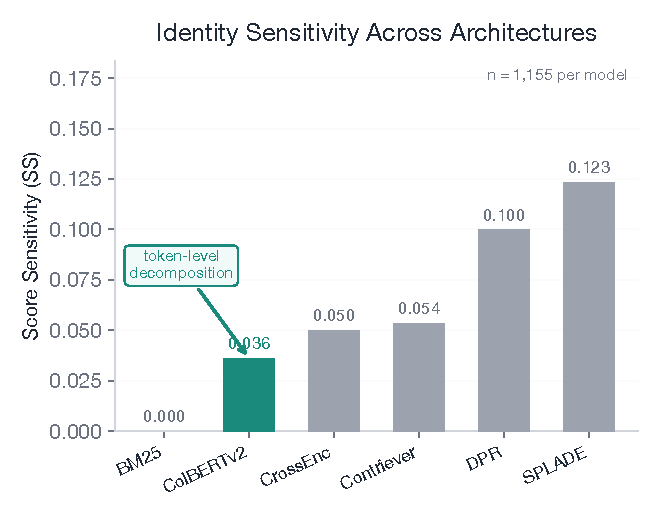
\includegraphics[width=\columnwidth]{figures/fig5_multi_model.pdf}
\caption{\textbf{Aggregate identity sensitivity across architectures.} Comparison of aggregate score sensitivity (SS) across different neural retrieval architectures ($n=1{,}155$ per model). While all models exhibit non-zero aggregate sensitivity, only ColBERT supports exact token-level decomposition.}
\label{fig:multimodel}
\end{figure}

\section{Computational Details}
\label{app:compute}

All models are publicly available under permissive licenses (MIT/Apache 2.0). ColBERTv2 uses a BERT-base backbone ($\sim$110M parameters). DPR ($\sim$110M), Contriever ($\sim$110M), SPLADE ($\sim$110M), and the cross-encoder MiniLM-L-6-v2 ($\sim$22M) are all run at inference only, with no fine-tuning or hyperparameter search.

All experiments were run on a single Apple M-series CPU (no GPU) in approximately 50 minutes total. The main ColBERT experiment (55{,}440 tests) takes $\sim$22 minutes; each multi-model comparison (1{,}155 tests) takes $\sim$5 minutes; the naturalistic-text validation (8{,}000 tests) takes $\sim$7 minutes. The 200-trial expanded synthetic ranking simulations and query-ablation probes add approximately 6 minutes of runtime. Runtime excludes optional plotting and bootstrap resampling.

\end{document}
